% Options for packages loaded elsewhere
\PassOptionsToPackage{unicode}{hyperref}
\PassOptionsToPackage{hyphens}{url}
\documentclass[
]{book}
\usepackage{xcolor}
\usepackage{amsmath,amssymb}
\setcounter{secnumdepth}{5}
\usepackage{iftex}
\ifPDFTeX
  \usepackage[T1]{fontenc}
  \usepackage[utf8]{inputenc}
  \usepackage{textcomp} % provide euro and other symbols
\else % if luatex or xetex
  \usepackage{unicode-math} % this also loads fontspec
  \defaultfontfeatures{Scale=MatchLowercase}
  \defaultfontfeatures[\rmfamily]{Ligatures=TeX,Scale=1}
\fi
\usepackage{lmodern}
\ifPDFTeX\else
  % xetex/luatex font selection
\fi
% Use upquote if available, for straight quotes in verbatim environments
\IfFileExists{upquote.sty}{\usepackage{upquote}}{}
\IfFileExists{microtype.sty}{% use microtype if available
  \usepackage[]{microtype}
  \UseMicrotypeSet[protrusion]{basicmath} % disable protrusion for tt fonts
}{}
\makeatletter
\@ifundefined{KOMAClassName}{% if non-KOMA class
  \IfFileExists{parskip.sty}{%
    \usepackage{parskip}
  }{% else
    \setlength{\parindent}{0pt}
    \setlength{\parskip}{6pt plus 2pt minus 1pt}}
}{% if KOMA class
  \KOMAoptions{parskip=half}}
\makeatother
\usepackage{longtable,booktabs,array}
\usepackage{calc} % for calculating minipage widths
% Correct order of tables after \paragraph or \subparagraph
\usepackage{etoolbox}
\makeatletter
\patchcmd\longtable{\par}{\if@noskipsec\mbox{}\fi\par}{}{}
\makeatother
% Allow footnotes in longtable head/foot
\IfFileExists{footnotehyper.sty}{\usepackage{footnotehyper}}{\usepackage{footnote}}
\makesavenoteenv{longtable}
\usepackage{graphicx}
\makeatletter
\newsavebox\pandoc@box
\newcommand*\pandocbounded[1]{% scales image to fit in text height/width
  \sbox\pandoc@box{#1}%
  \Gscale@div\@tempa{\textheight}{\dimexpr\ht\pandoc@box+\dp\pandoc@box\relax}%
  \Gscale@div\@tempb{\linewidth}{\wd\pandoc@box}%
  \ifdim\@tempb\p@<\@tempa\p@\let\@tempa\@tempb\fi% select the smaller of both
  \ifdim\@tempa\p@<\p@\scalebox{\@tempa}{\usebox\pandoc@box}%
  \else\usebox{\pandoc@box}%
  \fi%
}
% Set default figure placement to htbp
\def\fps@figure{htbp}
\makeatother
\setlength{\emergencystretch}{3em} % prevent overfull lines
\providecommand{\tightlist}{%
  \setlength{\itemsep}{0pt}\setlength{\parskip}{0pt}}
\usepackage[]{natbib}
\bibliographystyle{plainnat}
\usepackage{booktabs}
\usepackage{booktabs}
\usepackage{longtable}
\usepackage{array}
\usepackage{multirow}
\usepackage{wrapfig}
\usepackage{float}
\usepackage{colortbl}
\usepackage{pdflscape}
\usepackage{tabu}
\usepackage{threeparttable}
\usepackage{threeparttablex}
\usepackage[normalem]{ulem}
\usepackage{makecell}
\usepackage{xcolor}
\usepackage{bookmark}
\IfFileExists{xurl.sty}{\usepackage{xurl}}{} % add URL line breaks if available
\urlstyle{same}
\hypersetup{
  pdftitle={Statistics For Science Extension},
  pdfauthor={Michael Dear},
  hidelinks,
  pdfcreator={LaTeX via pandoc}}

\title{Statistics For Science Extension}
\author{Michael Dear}
\date{2026-03-19}

\begin{document}
\maketitle

{
\setcounter{tocdepth}{1}
\tableofcontents
}
\part*{Part 1: Statistical Concepts}\label{part-part-1-statistical-concepts}
\addcontentsline{toc}{part}{Part 1: Statistical Concepts}

\chapter{Introduction}\label{introduction}

\begin{quote}
\textbf{Learning Objectives}\\
To define statistics and its purpose\\
To review the process and design of scientific studies\\
To understand the difference between populations and samples\\
To understand the difference between descriptive and inferential statistics
\end{quote}

These notes are a practical introduction to statistics for students of the NSW Science Extension course. The emphasis is on learning through examples and problem-solving.

\section{What Is Statistics and What Does It Do?}\label{what-is-statistics-and-what-does-it-do}

There is no one simple definition for what statistics is and what it does.

``Statistics uses samples to explain and predict''

``Statistics is a set of techniques for collecting and analysing data''

``Statistics tells the story of the population being studied''

However, it can be said that statistics is fundamental to all stages of scientific research.

\section{Examples of Statistical Problems}\label{examples-of-statistical-problems}

Most scientific research questions will rely heavily on statistical techniques:

\begin{itemize}
\tightlist
\item
  What is the average girth (circumference) of trees in a forest?
\item
  What is the rate of decline in seabird populations in Australian coastal waters?
\item
  Does a new vaccine reduce the number of deaths from influenza?
\item
  Predict the rise in temperature by 2050 in different regions of Australia.
\end{itemize}

\section{A More Detailed Example}\label{a-more-detailed-example}

Forestry scientists would like to know the average girth (circumference) of trees in a forest. There are too many trees to measure them all, so they plan to take a random sample of 200 trees. They need to use statistics to determine the size and structure of the sample. After collecting the data, they complete a statistical analysis to estimate that, to a high level of confidence, the average tree girth is between 175cm and 225cm. They then write a report using statistical tables and plots to communicate their results.

\section{Scientific Studies}\label{scientific-studies}

A scientific study has the following steps:

\begin{itemize}
\tightlist
\item
  Research question(s)
\item
  Study design - experimental or observational?
\item
  Data collection
\item
  Data analysis
\item
  Report
\end{itemize}

\section{Study Design}\label{study-design}

There are two basic types of scientific study:

\begin{quote}
\textbf{Observational study} - variables are not controlled e.g.~the health records of 1000 people who had taken Drug X were reviewed to determine the side effects.
\end{quote}

\begin{quote}
\textbf{Experimental study} - variables are controlled e.g.~Plots A and B are next to each other. Plot A receives fertiliser and Plot B receives none.
\end{quote}

Observational studies can show \emph{associations} between variables, but experimental studies can show \emph{causal} relationships.

\begin{quote}
Observational study \(\rightarrow\) association - ``A varies as B varies''\\
Experimental study \(\rightarrow\) causation - ``A causes B''
\end{quote}

\section{Population and Sample}\label{population-and-sample}

\begin{quote}
\textbf{Population} - all members of the group being studied e.g.~all the Magpies in NSW. Population values are called \textbf{parameters}.
\end{quote}

\begin{quote}
\textbf{Sample} - a subset of the population being studied e.g.~1000 magpies chosen at random locations across NSW. Sample values are called \textbf{statistics}.
\end{quote}

\section{Symbols For Common Values}\label{symbols-for-common-values}

\begin{longtable}[]{@{}lll@{}}
\toprule\noalign{}
Value & Population Parameter & Sample Statistic \\
\midrule\noalign{}
\endhead
\bottomrule\noalign{}
\endlastfoot
Mean & \(\mu\) & \(\bar{x}\) \\
Standard Deviation & \(\sigma\) & \(s\) \\
Proportion & \(p\) & \(\hat{p}\) \\
\end{longtable}

\section{Descriptive and Inferential Statistics}\label{descriptive-and-inferential-statistics}

\begin{quote}
\textbf{Descriptive statistics} describe data e.g.~mean, median, standard deviation of a data set.
\end{quote}

\begin{quote}
\textbf{Inferential statistics} estimate population parameters from a sample.
\end{quote}

Statistical analysis usually begins with descriptive statistics, then moves on to inferential statistics.

\begin{center}\rule{0.5\linewidth}{0.5pt}\end{center}

\section{Extension - Spreadsheets and Statistical Computing Languages}\label{extension---spreadsheets-and-statistical-computing-languages}

Spreadsheets are handy for recording and exploring small data sets. However, the capabilities of spreadsheets for statistical analysis are limited. Larger projects are best completed using a statistical computing language such as R. Analyses completed using computer coding have many advantages, such as

\begin{itemize}
\tightlist
\item
  the ability to handle very large data sets
\item
  a greater variety of plots
\item
  greater control over plot and data output
\item
  the availability of sophisticated modelling techniques
\item
  a coding script becomes a reproducible record of the steps completed during the project
\end{itemize}

The disadvantage of coding is the time taken to learn a language, although there are numerous training resources and forums available for free on the internet.

These notes, including plots, tables, and most diagrams, were created using the R statistical computing language.

\begin{center}\rule{0.5\linewidth}{0.5pt}\end{center}

\section{Activity}\label{activity}

Write definitions for each term:

\begin{itemize}
\tightlist
\item
  Population
\item
  Parameter
\item
  Sample
\item
  Statistic
\item
  Experimental study
\item
  Causation
\item
  Observational study
\item
  Association
\item
  Descriptive statistics
\item
  Inferential statistics
\end{itemize}

\chapter{Data Concepts}\label{data_concepts}

\begin{quote}
\textbf{Learning Objectives}\\
To uderstand the basic types of data\\
To understand how data is structured for statistical analysis\\
To determine the amount of data required for a scientific study\\
To investigate methods of data collection\\
To distinguish between primary and secondary sources\\
To review some secondary sources of scientific data\\
To learn the steps in preparing data for statistical analysis
\end{quote}

\section{Types of Data}\label{types-of-data}

\begin{figure}
\centering
\pandocbounded{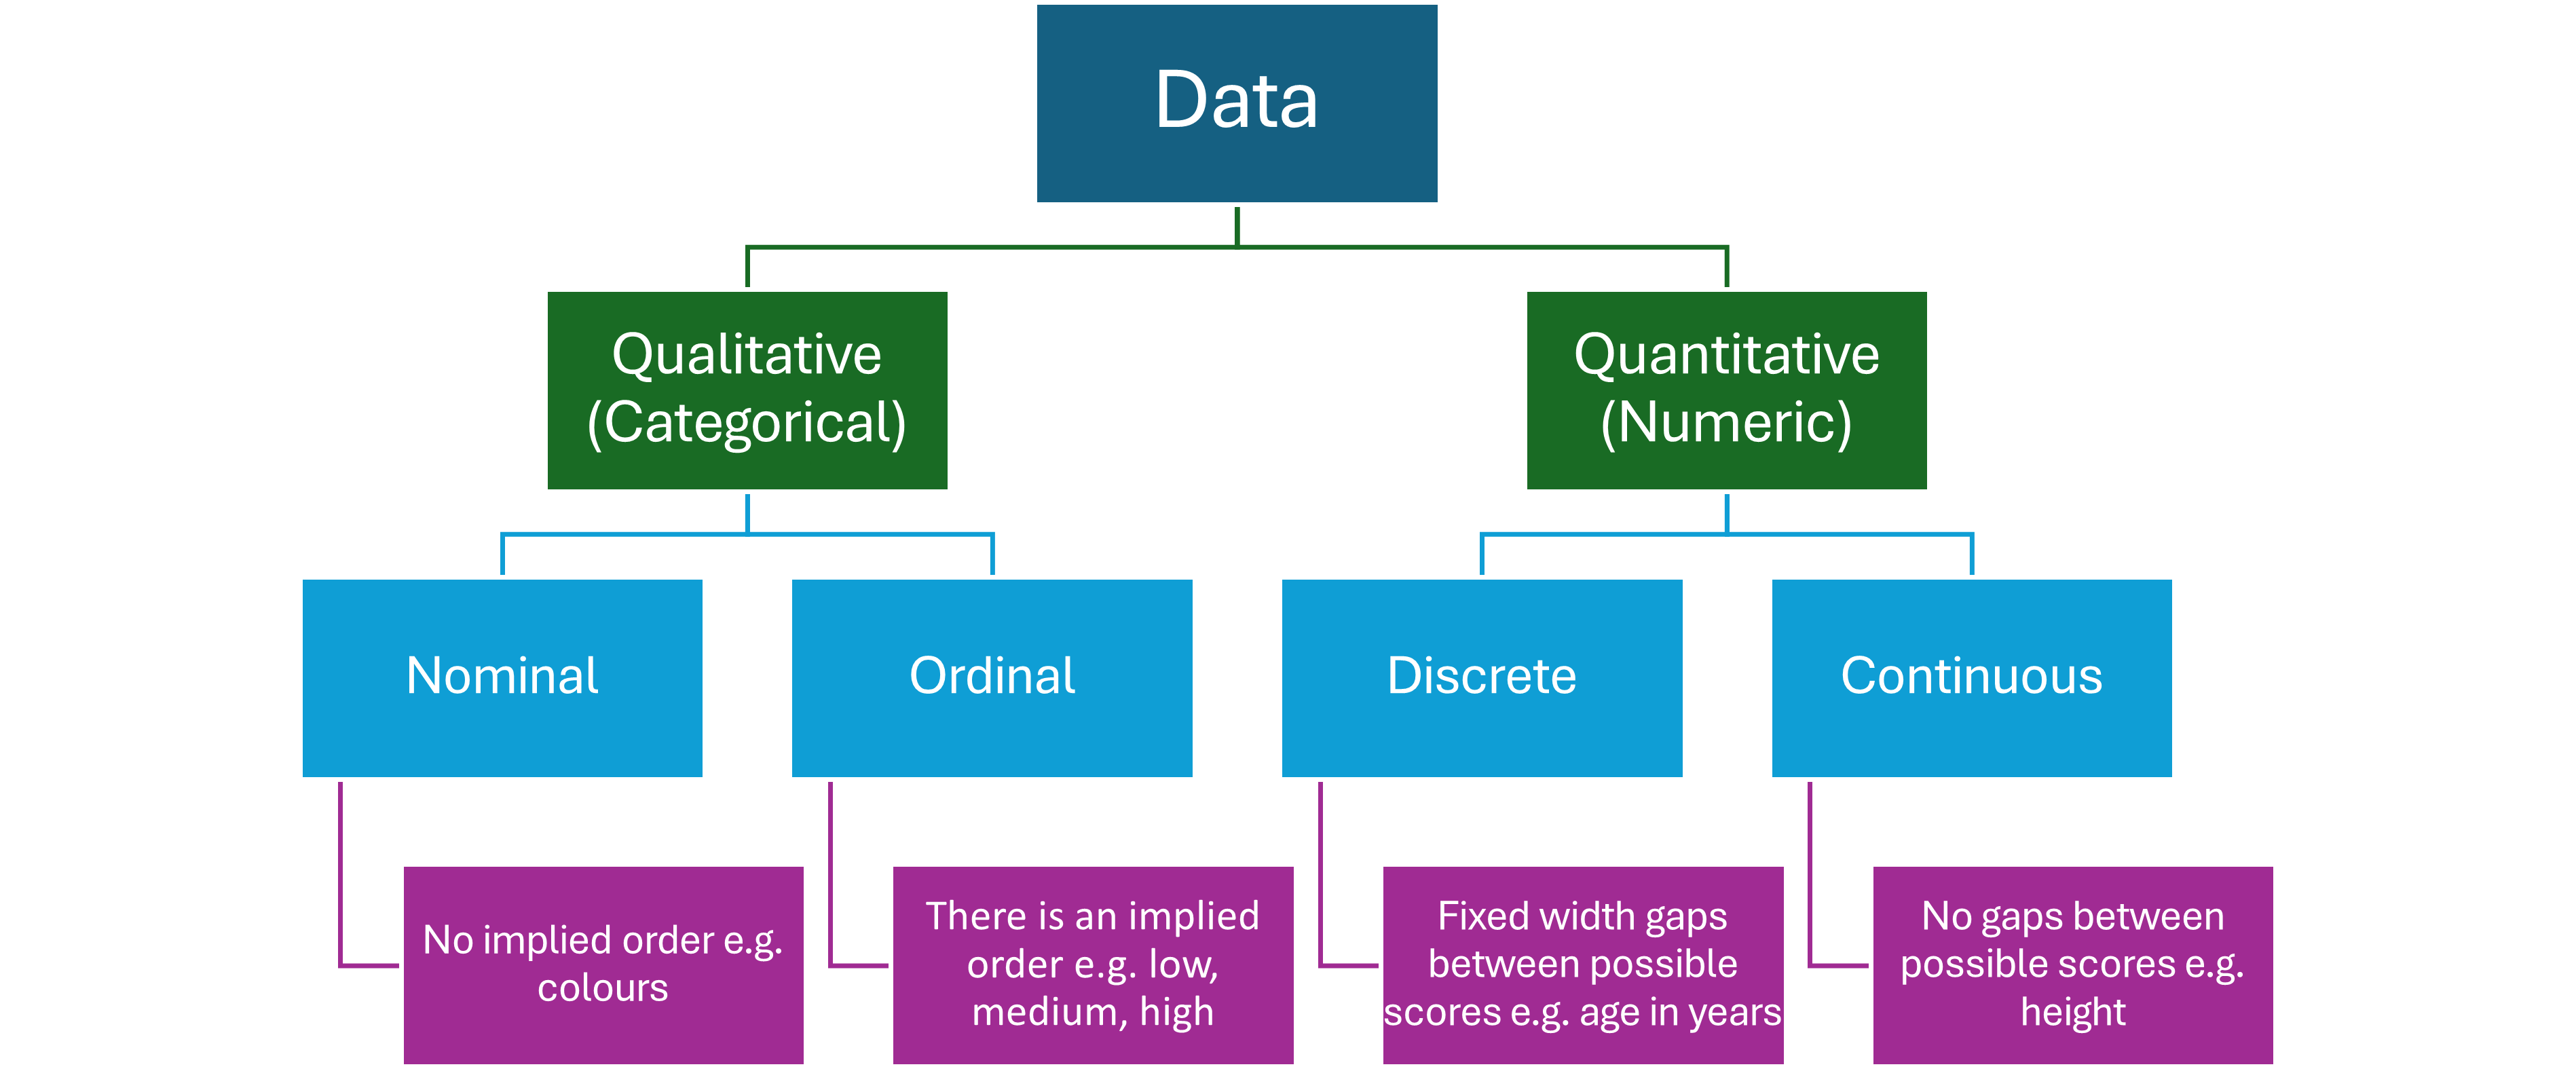
\includegraphics[keepaspectratio]{./resources/img/types_of_data.png}}
\caption{The basic types of data.}
\end{figure}

\begin{quote}
\emph{Count data} is quantitative discrete data in which the number of occurrences of something are recorded e.g.~the number of birds in migratory flocks.
\end{quote}

\begin{quote}
\emph{Qualitative} data is often described as a \emph{grouping variable} e.g.~the participants in a medical trial are grouped by the treatment they are given.
\end{quote}

\section{The Structure of Data}\label{the-structure-of-data}

Data should be structured using tables in which

\begin{itemize}
\tightlist
\item
  each column represents a variable
\item
  the values in each column are the same type and the same unit
\item
  the first row contains the names of the variables without any spaces
\end{itemize}

The data in each row represents a single \emph{observation} of the variables. Observations are often called \emph{records} or \emph{cases}, depending on the context of the study. Similarly, columns are often called \emph{attributes}, \emph{features} or \emph{fields}.

\subsection{File Formats For Data Storage and Exchange}\label{file-formats-for-data-storage-and-exchange}

The most common format for storing and exchanging data for statistical analysis is \emph{comma separated format} (CSV). CSV is a plain text file with fields separated by commas. Numeric data is unquoted and text data is surrounded by quotation marks. CSV files usually have the extension ``.csv''.

The following is an example of CSV file contents. The first row is the column headers, and the remaining rows are observations.

\begin{verbatim}
"Sepal.Length","Sepal.Width","Petal.Length","Petal.Width","Species"
5.1,3.5,1.4,0.2,"setosa"
4.9,3,1.4,0.2,"setosa"
4.7,3.2,1.3,0.2,"setosa"
\end{verbatim}

\subsection{Activity}\label{activity-1}

\begin{enumerate}
\def\labelenumi{\arabic{enumi}.}
\tightlist
\item
  List the variables and the type of data they represent for the following data set.
\item
  Write down one observation from the table.
\end{enumerate}

\begin{verbatim}
 Sepal.Length Sepal.Width Petal.Length Petal.Width    Species
          5.9         3.0          5.1         1.8  virginica
          5.5         4.2          1.4         0.2     setosa
          7.1         3.0          5.9         2.1  virginica
          6.3         2.8          5.1         1.5  virginica
          5.8         2.6          4.0         1.2 versicolor
          5.8         4.0          1.2         0.2     setosa
\end{verbatim}

\section{Collecting Data}\label{collecting-data}

Data sources can be classified as either \emph{primary} or \emph{secondary}.

\begin{quote}
\textbf{Primary Source Data} is collected by the researcher through first-hand surveys.\\
\textbf{Secondary Source Data} is collected from existing data repositories.
\end{quote}

\subsection{Sample Size - How Much Data Is Enough?}\label{sample-size---how-much-data-is-enough}

Estimating the sample size for a research project is important because

\begin{itemize}
\tightlist
\item
  sample size needs to be large enough to detect the expected effect if it's present
\item
  a sample that is too large is wasteful of resources or could be unethical
\item
  the study might not be feasible if a large sample size is required.
\end{itemize}

Estimating sample size depends on

\begin{itemize}
\tightlist
\item
  the objective(s) of the research
\item
  the type of statistical tests or modelling that will be applied
\item
  the type of study design e.g.~experimental versus observational studies
\item
  if the target outcome is a rare case
\end{itemize}

Sample size can be estimated using software tools or, for situations where less scientific rigor is required, by ``rules of thumb''.

\begin{center}\rule{0.5\linewidth}{0.5pt}\end{center}

\subsection{Extension}\label{extension}

You might come across them in your research when estimating the sample size required for your project.

\begin{quote}
\textbf{Definitions}
\textbf{Type I Error} - rejecting a true null hypothesis (false positive - accepting there is a significant effect when there isn't one)\\
\textbf{Type II Error} - not rejecting a false null hypothesis (false negative - missing a significant effect when there is one)\\
\textbf{Power} - the ability of a statistical test to detect an effect given that the effect exists. Formal definition: \(\text{Power} = 1 - \text{P(Type II Error)}\)
\end{quote}

We will come back to hypothesis testing in a later lesson.

\begin{center}\rule{0.5\linewidth}{0.5pt}\end{center}

\subsection{Large Data Sets}\label{large-data-sets}

Large data sets have become commonplace since the advent of the internet and increasingly powerful computers. While these data sets provide the ability to work with very large samples, they introduce the problem of ``information overload''. Too much data can be as big a problem as too little data!

To overcome some of the problems associated with large data sets, they are increasingly available online along with the ability to process the data using cloud computing. This makes the task of working with large data sets more achievable for individuals and smaller institutions.

\subsection{Activity - Online Data Repositories}\label{activity---online-data-repositories}

Explore the following data repositories and complete the table.

\begin{longtable}[]{@{}
  >{\raggedright\arraybackslash}p{(\linewidth - 6\tabcolsep) * \real{0.2083}}
  >{\raggedright\arraybackslash}p{(\linewidth - 6\tabcolsep) * \real{0.1875}}
  >{\raggedright\arraybackslash}p{(\linewidth - 6\tabcolsep) * \real{0.1458}}
  >{\raggedright\arraybackslash}p{(\linewidth - 6\tabcolsep) * \real{0.4583}}@{}}
\toprule\noalign{}
\begin{minipage}[b]{\linewidth}\raggedright
Repository
\end{minipage} & \begin{minipage}[b]{\linewidth}\raggedright
Main Uses
\end{minipage} & \begin{minipage}[b]{\linewidth}\raggedright
Formats
\end{minipage} & \begin{minipage}[b]{\linewidth}\raggedright
Cloud Processing (y/n)
\end{minipage} \\
\midrule\noalign{}
\endhead
\bottomrule\noalign{}
\endlastfoot
\href{https://www.abs.gov.au/}{ABS} & & & \\
\href{https://data.gov.au/}{data.gov.au} & & & \\
\href{https://www.seed.nsw.gov.au/}{SEED NSW} & & & \\
\href{https://www.ga.gov.au/scientific-topics/dea}{Digital Earth Australia} & & & \\
\href{https://www.ala.org.au/}{Atlas of Living Australia} & & & \\
\end{longtable}

\section{Data Cleaning}\label{data-cleaning}

Most data needs preparation or ``cleaning'' before statistical analysis can begin.

There is an expression that says ``10 percent inspiration, 90 percent perspiration''. In the case of statistics, preparing data for analysis is often the ``90 percent perspiration''! Most real-world data sets will need a lot of cleaning before they are suitable for use in a research project.

Some of the issues that need to be checked and remedied are

\begin{itemize}
\tightlist
\item
  missing values, often labelled as \textbf{NA}, but might just be blank - impute, drop, or ignore?
\item
  incorrect number formats e.g.~differing numbers of decimal places, missing decimal points: 1.02, 1.15, 103, 1.96
\item
  units included in quantitative columns e.g.~9.1, 3.2, 5.8mm, 6.7
\item
  Not the correct number of rows e.g.~your data set should have 1000 rows, but it only has 100 when you open it
\item
  duplicate categories in qualitative variables e.g.~dog, cat, cat, dogs, cats
\item
  dates and times are not recognised correctly by the software
\item
  outliers
\item
  duplicate records
\item
  removing irrelevant variables; finding the relevant ones amongst hundreds
\item
  variables that have only one value or are empty
\item
  column names that contain characters not permitted in some computing languages e.g.~\%, \#, \$
\item
  columns that have no name
\item
  metadata added at the beginning or end of data tables exported from secondary sources - always check the end of the data for unwanted additions!
\item
  empty rows, cells, merged cells in spreadsheets :(
\end{itemize}

\ldots{} and the list goes on.

\begin{quote}
\textbf{Tip}\\
For a small project where you are working alone or in a small team, avoid most of these problems by developing a thorough plan and keeping accurate records. Do not change your methods once you have started recording data.
\end{quote}

\subsection{Activity}\label{activity-2}

Open the \href{resources/datasets/messy_data.csv}{messy\_data.csv} data set in a spreadsheet. This data represents observations from a national wildlife database for a study area. Find any issues with the data and decide what should be done to prepare the data for analysis.

\chapter{Exploratory Data Analysis}\label{eda}

\begin{quote}
\textbf{Learning Objectives}\\
To review common descriptive statistics\\
To review common statistical plots\\
To perform exploratory data analysis using a spreadsheet
\end{quote}

Once the study has been designed and data collected, it's time to begin analysing the results. The first step in analysis is getting to know the data set. The steps of exploratory data analysis (EDA) include

\begin{itemize}
\tightlist
\item
  summarising quantitative variables - n, min, max, quartiles, mean, standard deviation
\item
  using boxplots and histograms to investigate spread and skewness
\item
  using scatter plots to investigate associations between quantitative variables
\item
  using grouping variables to investigate the similarities and differences between groups
\end{itemize}

The following descriptive statistics and plots use the well-known Iris data set. The data set contains measurements of flower parts for three species of Iris.

\section{Common Descriptive Statistics}\label{common-descriptive-statistics}

\begin{quote}
\textbf{Definitions}\\
\textbf{n} - the number of scores\\
\textbf{Minimum (min)} - lowest score\\
\textbf{Maximum (max)} - highest score\\
\textbf{Quartiles} - the scores that break the data into quarters - Q1 25\%; Q2 50\% (Median); Q3 75\%\\
\textbf{Mean} - the average; sum of scores divided by number of scores\\
\textbf{Standard Deviation (sd)} - average distance of scores from the mean
\end{quote}

When approaching a new data set, a good first step is to determine the data type of each variable (column).

\begin{verbatim}
Rows: 150
Columns: 5
$ Sepal.Length <dbl> 5.1, 4.9, 4.7, 4.6, 5.0, 5.4, 4.6, 5.0, 4.4, 4.9, 5.4, 4.~
$ Sepal.Width  <dbl> 3.5, 3.0, 3.2, 3.1, 3.6, 3.9, 3.4, 3.4, 2.9, 3.1, 3.7, 3.~
$ Petal.Length <dbl> 1.4, 1.4, 1.3, 1.5, 1.4, 1.7, 1.4, 1.5, 1.4, 1.5, 1.5, 1.~
$ Petal.Width  <dbl> 0.2, 0.2, 0.2, 0.2, 0.2, 0.4, 0.3, 0.2, 0.2, 0.1, 0.2, 0.~
$ Species      <fct> setosa, setosa, setosa, setosa, setosa, setosa, setosa, s~
\end{verbatim}

The output above shows that the Iris data set has five variables, four that are continuous (\emph{\textless dbl\textgreater{}}) and one that is qualitative (\emph{\textless fct\textgreater{}}). There are 150 records (rows) in the data set.

The following is a summary of descriptive statistics for each variable in the Iris data set.

\begin{table}

\caption{\label{tab:unnamed-chunk-4}Summary Statistics}
\centering
\begin{tabular}[t]{llllllllll}
\toprule
Variable & notNA & NA & Mean & SD & Min & Q1 & Median & Q2 & Max\\
\midrule
Sepal.Length & 150 & 0 & 5.8 & 0.83 & 4.3 & 5.1 & 5.8 & 6.4 & 7.9\\
Sepal.Width & 150 & 0 & 3.1 & 0.44 & 2 & 2.8 & 3 & 3.3 & 4.4\\
Petal.Length & 150 & 0 & 3.8 & 1.8 & 1 & 1.6 & 4.3 & 5.1 & 6.9\\
Petal.Width & 150 & 0 & 1.2 & 0.76 & 0.1 & 0.3 & 1.3 & 1.8 & 2.5\\
\bottomrule
\end{tabular}
\end{table}

\begin{quote}
\textbf{Question}\\
What are some conclusions that you can draw about the data set from the above summary?
\end{quote}

\begin{quote}
\textbf{Table Formatting For Reports}\\
The previous table is an example of an appropriate way to format tables for scientific reports. See the \href{https://apastyle.apa.org/style-grammar-guidelines/tables-figures/tables}{APA tables webpage} for further details and examples.
\end{quote}

\section{Common Statistical Plots}\label{common-statistical-plots}

In school we usually use the word ``graph'', but statisticians usually use the word ``plot''. Spreadsheets call them ``charts''.

\subsection{Statistical Plot Summary}\label{stat_plot_summary}

\begin{longtable}[]{@{}
  >{\raggedright\arraybackslash}p{(\linewidth - 4\tabcolsep) * \real{0.2353}}
  >{\raggedright\arraybackslash}p{(\linewidth - 4\tabcolsep) * \real{0.5294}}
  >{\raggedright\arraybackslash}p{(\linewidth - 4\tabcolsep) * \real{0.2353}}@{}}
\toprule\noalign{}
\begin{minipage}[b]{\linewidth}\raggedright
Plot
\end{minipage} & \begin{minipage}[b]{\linewidth}\raggedright
Variables
\end{minipage} & \begin{minipage}[b]{\linewidth}\raggedright
Uses
\end{minipage} \\
\midrule\noalign{}
\endhead
\bottomrule\noalign{}
\endlastfoot
Boxplot & One quantitative variable; one grouping variable & Compares spread within groups; identifies outliers \\
Histogram & One continuous variable & Identifying the population distribution \\
Scatter Plot & Two continuous variables & Identifying relationships between variables e.g.~linear, non-linear; identifies outliers \\
Line Plot & One continuous variable; time with regular intervals & Observing change over time \\
\end{longtable}

\subsection{Boxplot}\label{boxplot}

Boxplots are used to

\begin{itemize}
\tightlist
\item
  show the distribution of data for each quartile of a quantitative variable.
\item
  identify outliers
\item
  compare groups
\end{itemize}

\begin{figure}
\centering
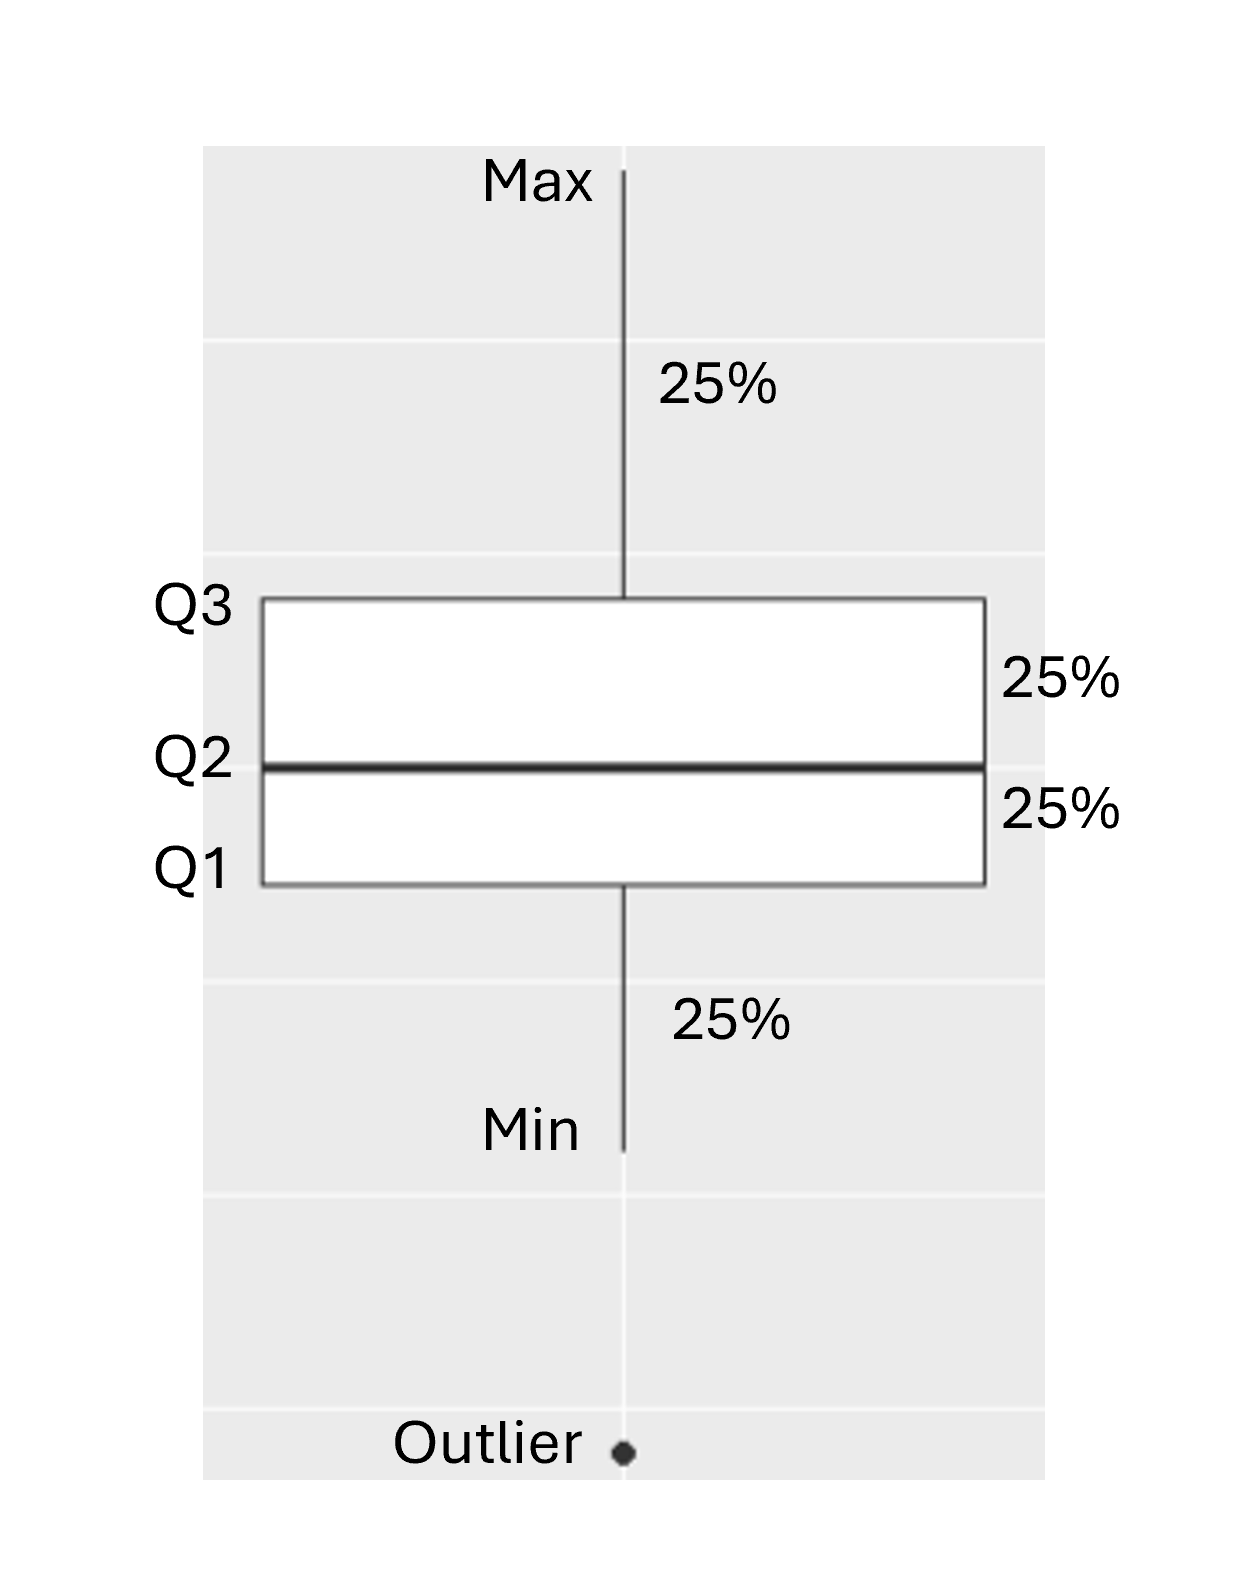
\includegraphics[width=0.5\linewidth,height=\textheight,keepaspectratio]{./resources/img/boxplot_diagram.png}
\caption{The structure of a boxplot.}
\end{figure}

The following boxplots show the distribution of Sepal Length grouped by species.

\pandocbounded{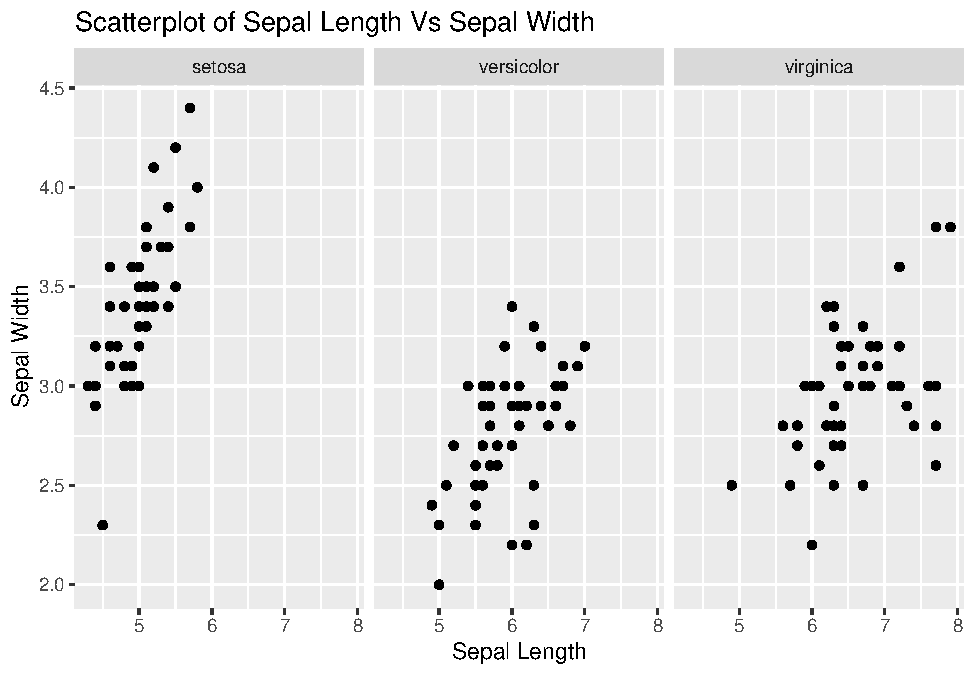
\includegraphics[keepaspectratio]{statistics_for_science_extension_files/figure-latex/unnamed-chunk-5-1.pdf}}

\begin{quote}
\textbf{Questions}\\
1. What do the thicker black lines inside the boxes represent?\\
2. What is similar and what is different about the three boxplots? Think in terms of spread and skewness.
\end{quote}

\subsection{Histogram}\label{histogram}

Histograms are used to help identify the type of distribution from which the data was drawn.

\pandocbounded{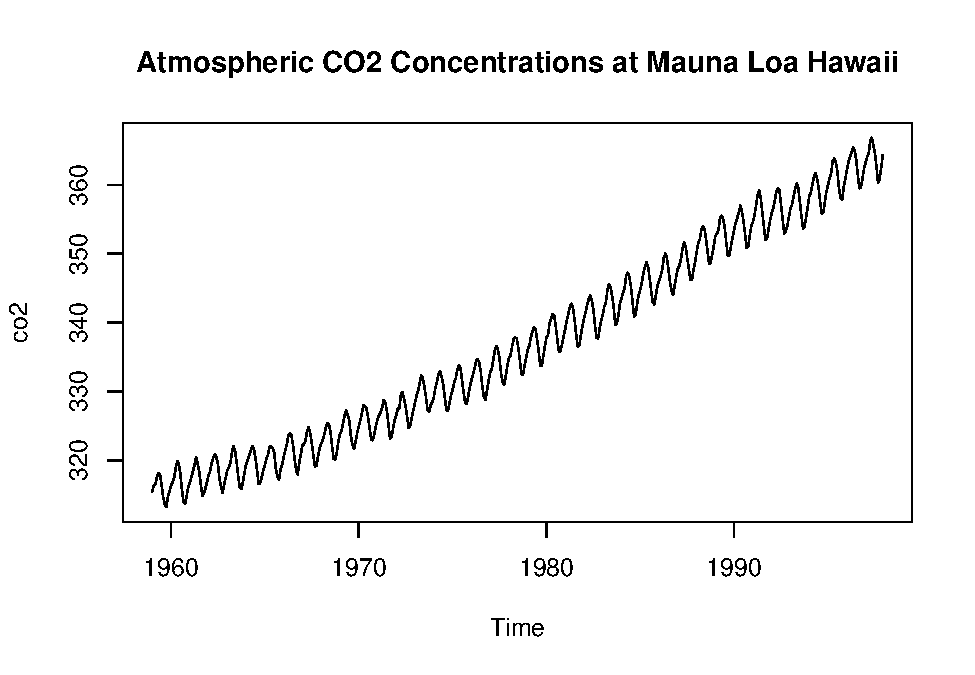
\includegraphics[keepaspectratio]{statistics_for_science_extension_files/figure-latex/unnamed-chunk-6-1.pdf}}

The histograms confirm that the distribution of Sepal.Length is approximately symmetrical for each species. This suggests that a normal distribution might be an appropriate model in each case. Also notice that there is an outlier in the virginica species, as was identified by the boxplot.

\subsection{Scatter Plot}\label{scatter-plot}

Scatter plots identify relationships between quantitative variables. If the relationship is linear, it is usually described in terms of the strength of the correlation and the direction of the relationship e.g.~``strong positive'' or ``moderate negative''.

\pandocbounded{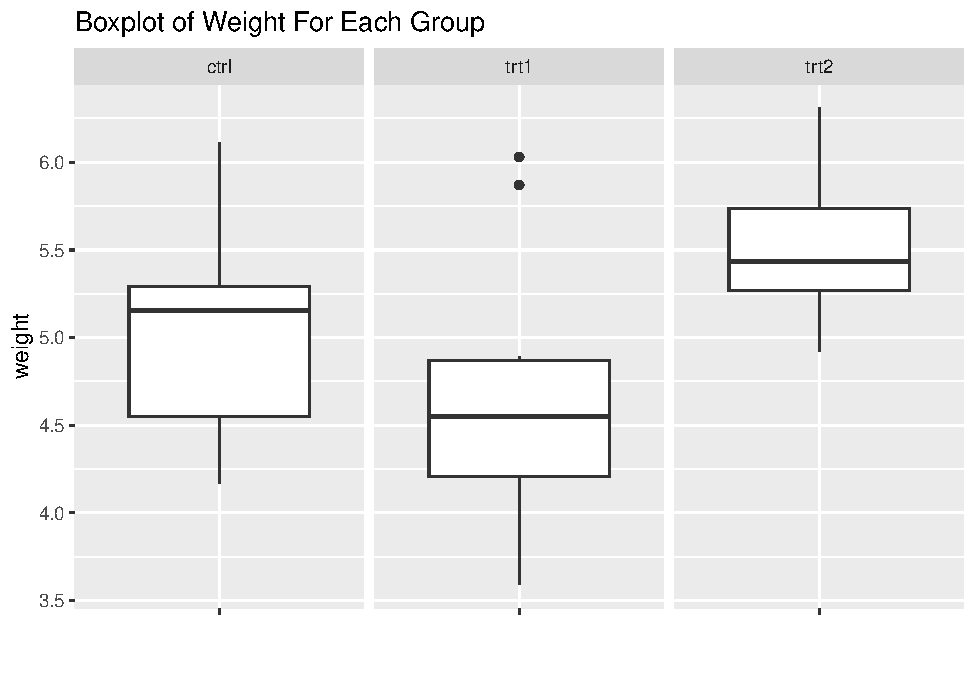
\includegraphics[keepaspectratio]{statistics_for_science_extension_files/figure-latex/unnamed-chunk-7-1.pdf}}

Scatter plots can also include a grouping (qualitative) variable using colour or different marker types. This can be useful for exploring relationships between different groups in the data set.

\pandocbounded{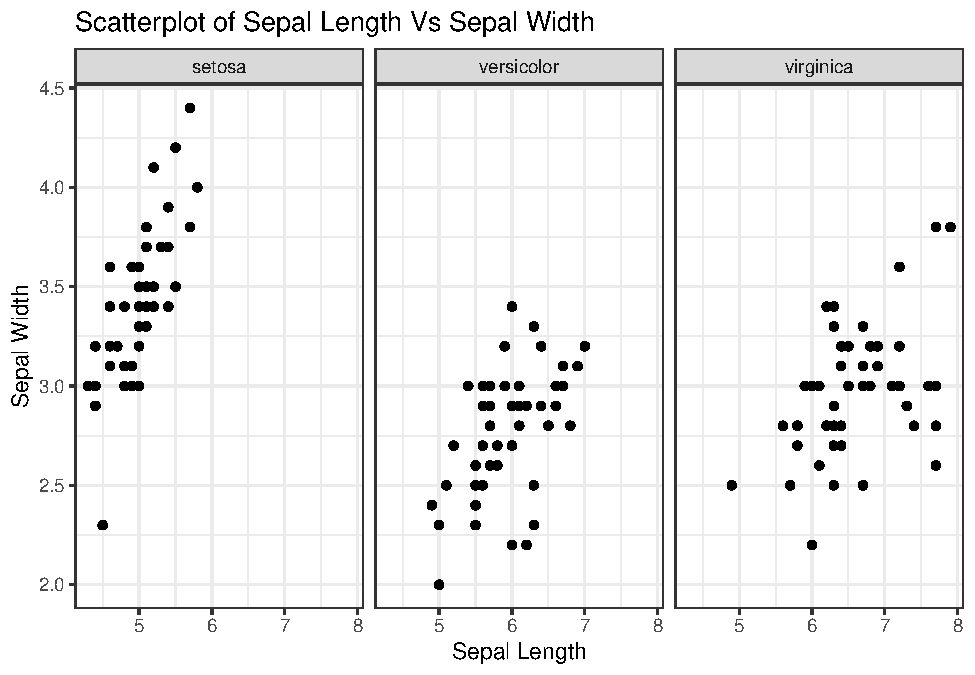
\includegraphics[keepaspectratio]{statistics_for_science_extension_files/figure-latex/unnamed-chunk-8-1.pdf}}

What extra insights are gained from the grouped plot when compared with the ungrouped plot?

\begin{quote}
\textbf{Questions}\\
1. Describe the relationship between Sepal Length and Sepal Width for each species.\\
2. Draw a line of fit onto each plot. Use this line to estimate the Sepal Width for a Sepal Length of 6.5 for each species.
\end{quote}

\subsection{Line Plot}\label{line-plot}

Line plots are often used for time series data e.g.~daily temperatures in March.

The following plot shows the concentration of atmospheric CO2 at Mauna Loa Hawaii.

\pandocbounded{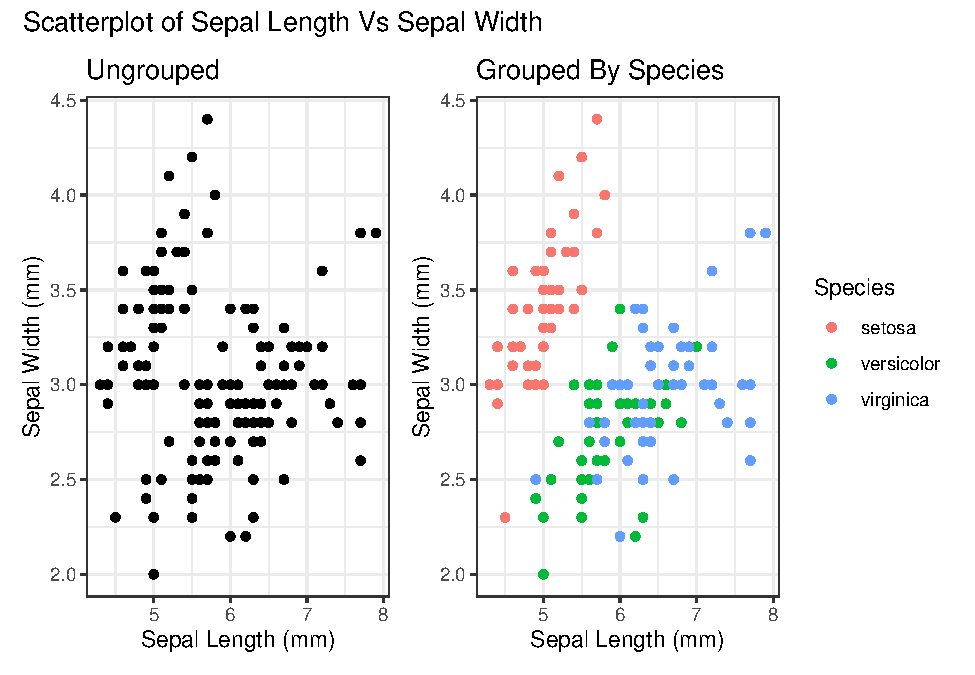
\includegraphics[keepaspectratio]{statistics_for_science_extension_files/figure-latex/unnamed-chunk-9-1.pdf}}

\begin{quote}
\textbf{Questions}\\
1. Describe the trend in the CO2 concentration.\\
2. Why does the plot zig-zag up and down?
\end{quote}

\begin{center}\rule{0.5\linewidth}{0.5pt}\end{center}

\subsection{Extension: Further Plots}\label{extension-further-plots}

\subsubsection{Points Plot}\label{points-plot}

This plot is similar to a scatter plot, except that the x-variable is qualitative. This plot shows the spread of each variable within each group of the qualitative variable.

\pandocbounded{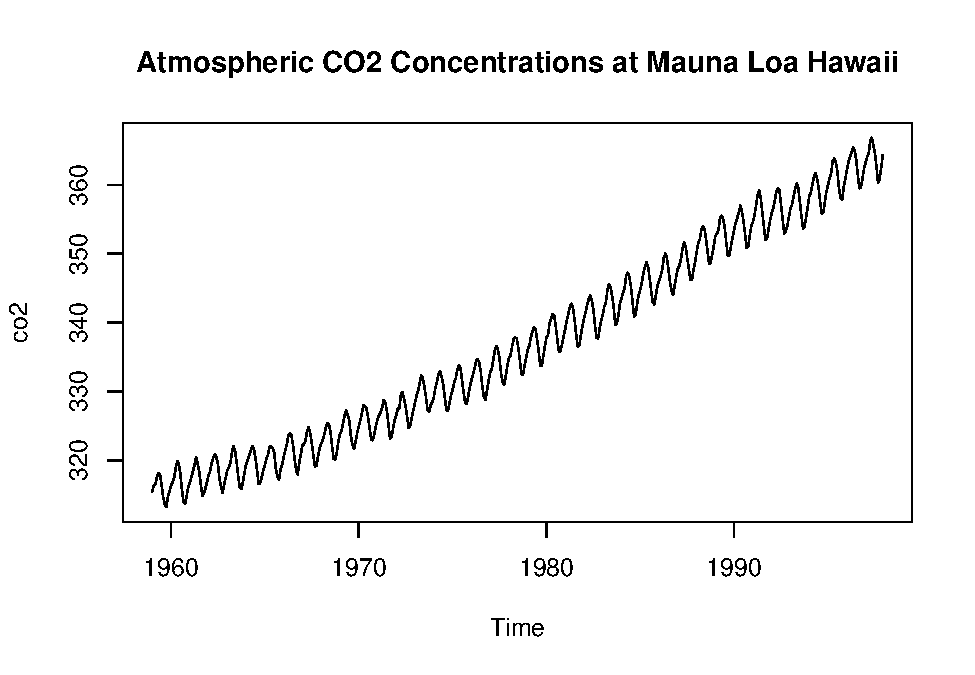
\includegraphics[keepaspectratio]{statistics_for_science_extension_files/figure-latex/unnamed-chunk-10-1.pdf}}

Overlaying the data points onto boxplots can provide useful additional information about the spread of the data.

\pandocbounded{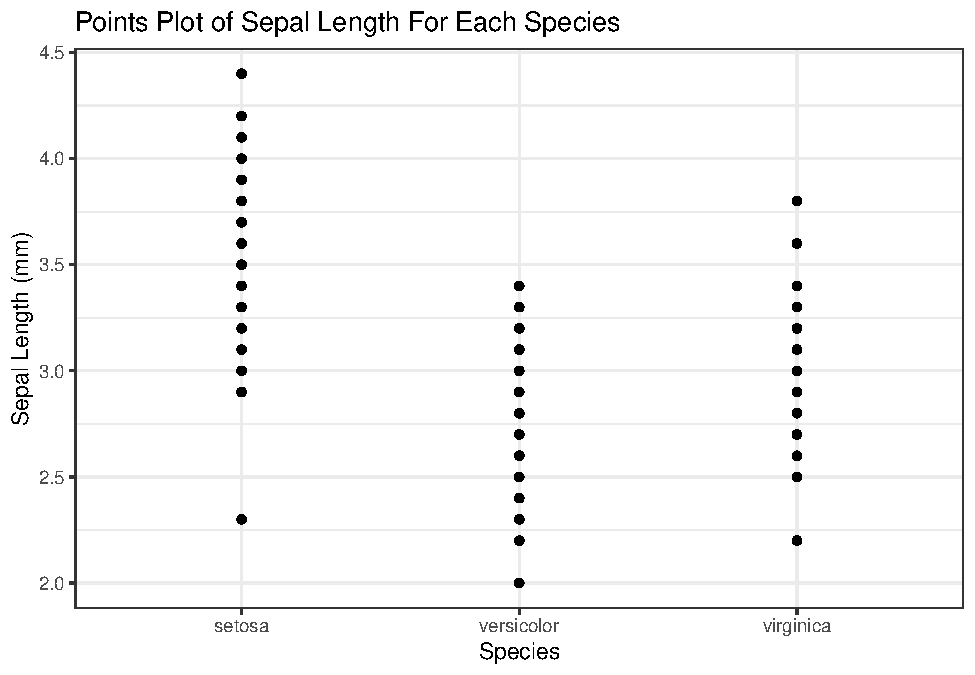
\includegraphics[keepaspectratio]{statistics_for_science_extension_files/figure-latex/unnamed-chunk-11-1.pdf}}

\begin{quote}
\textbf{Questions}\\
1. Estimate the mean for each species using the points plot.\\
2. Do you think there is a constant variance (standard deviation) for the three species?\\
3. Is there enough evidence in this sample to suggest that the population mean for Sepal Width is different for the three species? Why or why not?
\end{quote}

\subsubsection{Pairs}\label{pairs}

A pairs plot shows the relationships between all pairs of variables in a data set. This gives an overall picture of patterns within the data and is a useful tool for guiding research. The following plot includes scatter plots and correlation coefficients for quantitative pairs, boxplots for qualitative-quantitative pairs, and distribution curves for quantitative variables. Each plot has been coloured on the basis of species. To produce this type of plot requires statistical computing software such as R.

\pandocbounded{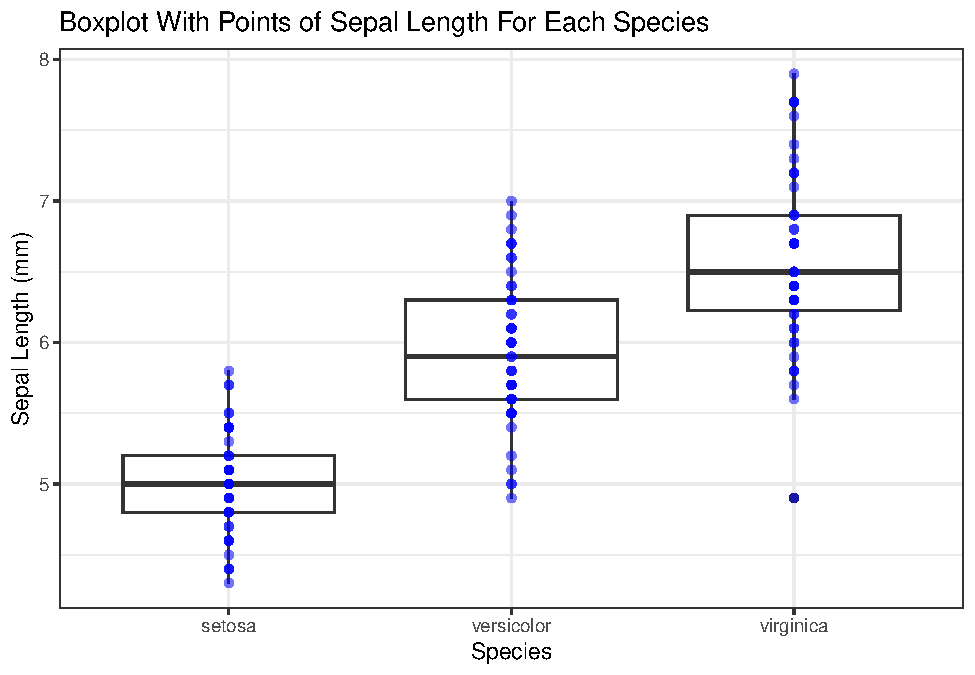
\includegraphics[keepaspectratio]{statistics_for_science_extension_files/figure-latex/unnamed-chunk-12-1.pdf}}

\begin{quote}
\textbf{Question}\\
1. Which variables show the greatest difference between the three species?
\end{quote}

\begin{center}\rule{0.5\linewidth}{0.5pt}\end{center}

\section{Activity}\label{activity-3}

Use the \href{resources/datasets/PlantGrowth.csv}{PlantGrowth} data set and a spreadsheet to

\begin{enumerate}
\def\labelenumi{\arabic{enumi}.}
\tightlist
\item
  Create a summary of the quantitative variable for each group including min, max, quantiles, mean, standard deviation
\item
  Create boxplots of the quantitative variable for each group in the data set.
\item
  Create histograms of the quantitative variable for each group in the data set.
\item
  Write a summary of your observations. Can you suggest any hypotheses?
\end{enumerate}

Hint: To make these plots and summaries in a spreadsheet, you will need to reorganise the data so there is one group per column.

\subsection{Solutions}\label{solutions}

\begin{verbatim}
Rows: 30
Columns: 2
$ weight <dbl> 4.17, 5.58, 5.18, 6.11, 4.50, 4.61, 5.17, 4.53, 5.33, 5.14, 4.8~
$ group  <fct> ctrl, ctrl, ctrl, ctrl, ctrl, ctrl, ctrl, ctrl, ctrl, ctrl, trt~
\end{verbatim}

\begin{verbatim}
# A tibble: 3 x 8
  group   Min    Q1 Median_Q2    Q3   Max  Mean    SD
  <fct> <dbl> <dbl>     <dbl> <dbl> <dbl> <dbl> <dbl>
1 ctrl   4.17  4.55      5.15  5.29  6.11  5.03 0.583
2 trt1   3.59  4.21      4.55  4.87  6.03  4.66 0.794
3 trt2   4.92  5.27      5.44  5.74  6.31  5.53 0.443
\end{verbatim}

\pandocbounded{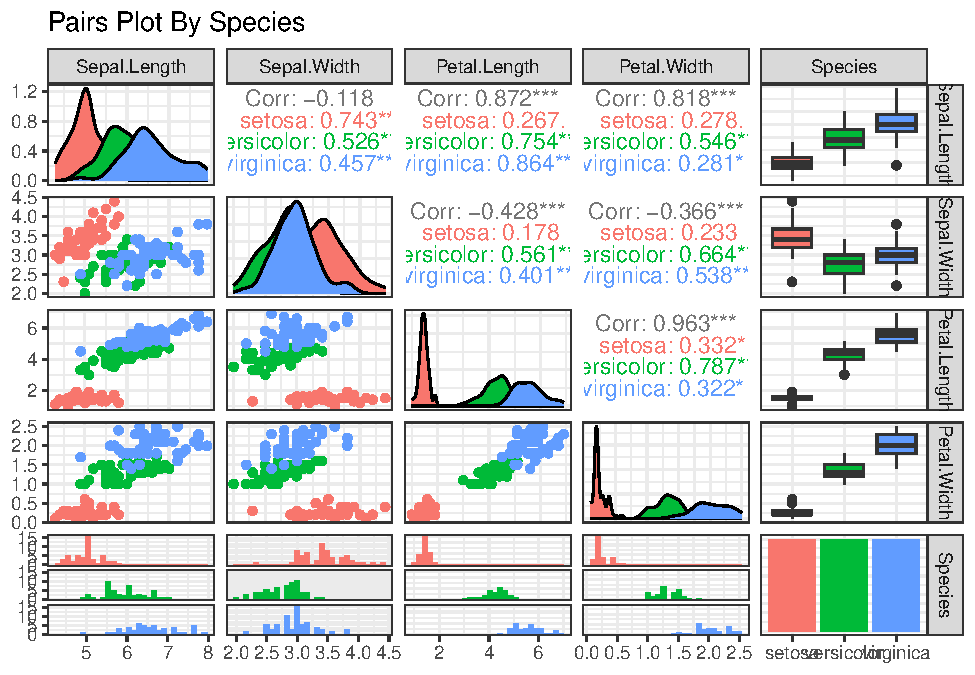
\includegraphics[keepaspectratio]{statistics_for_science_extension_files/figure-latex/unnamed-chunk-13-1.pdf}} \pandocbounded{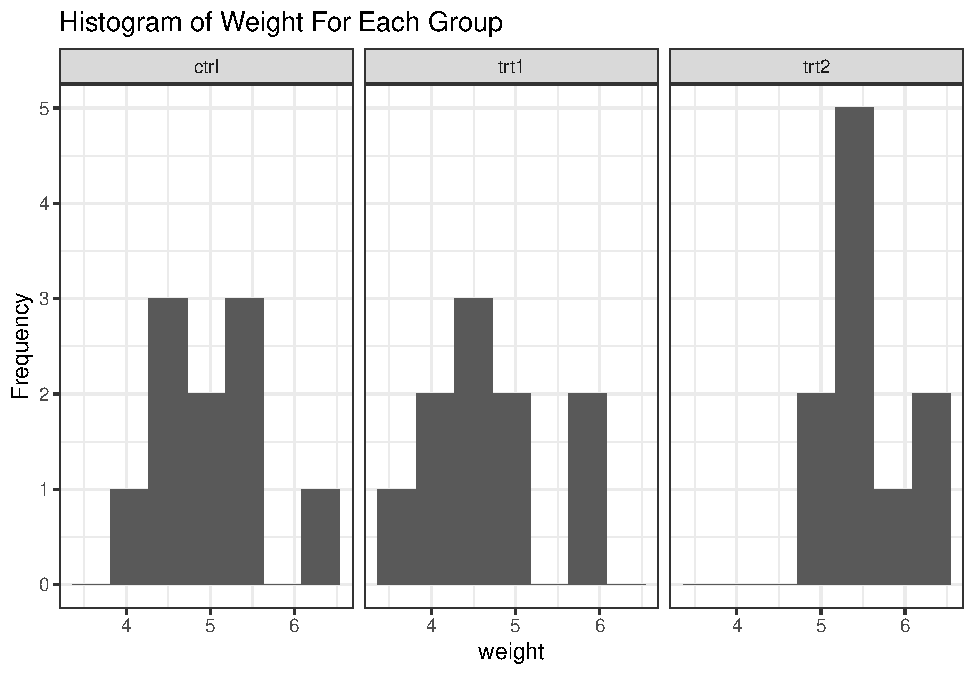
\includegraphics[keepaspectratio]{statistics_for_science_extension_files/figure-latex/unnamed-chunk-13-2.pdf}}

The ctrl group is slightly negatively skewed (Mean = 5.032 versus Median = 5.155). The greatest variation occurs on the trt1 group (SD = 0.79), and the least in the trt2 group (SD = 0.44). The boxplots show that the trt1 group has potential outliers at the upper values.

\chapter{Statistical Tests}\label{stat_tests}

\begin{quote}
\textbf{Learning Objectives}\\
To understand the process of sampling\\
To select, apply, and interpret common statistical tests\\
To understand p-values and statistical signifiance\\
To create and interpret confidence intervals
\end{quote}

\section{Sampling}\label{sampling}

\begin{itemize}
\tightlist
\item
  Sampling should be done with replacement
\item
  Often not with replacement in practice - OK for large enough population
\item
  Sources of dependency - time, space
\item
  Common sampling mistakes
\end{itemize}

\section{Common Statistical Tests}\label{common-statistical-tests}

\subsection{Table}\label{table}

\subsection{Examples}\label{examples}

\section{p-values and Statistical Significance}\label{p-values-and-statistical-significance}

\begin{itemize}
\tightlist
\item
  What and why?
\item
  Correct interpretation
\item
  Effect size
\item
  How to report
\end{itemize}

\section{Confidence Intervals}\label{confidence-intervals}

\chapter{Further Reading}\label{further_reading}

\section{Books}\label{books}

\href{https://www.openintro.org/book/ahss/}{\textbf{Advanced High School Statistics 3rd Ed, Diez et al}}: A detailed and rigorous introduction to statistics that would suit advanced high school and undergraduate university students. The theory and applications of statistics are covered from collecting data through to inference and statistical tests. The book contains numerous exercise and examples to help students develop their knowledge and skills.

\href{https://stats.libretexts.org/Bookshelves/Introductory_Statistics/Introductory_Statistics_(Shafer_and_Zhang)}{\textbf{Introductory Statistics, Shafer and Zhang}}: Hosted on \href{https://libretexts.org/}{LibreTexts}, this is another thorough but accessible introduction to the theory and practice of statistics. The book begins with a detailed explanation of descriptive statistics and probability, and random variables. Later chapters cover sampling distributions, hypotheses, and hypothesis testing.

\section{Websites}\label{websites}

\href{https://www.abs.gov.au/statistics/understanding-statistics/statistical-terms-and-concepts}{\textbf{Australian Bureau of Statistics ``Statistical Terms and Concepts''}}: A comprehensive glossary of statistical terms. Click the terms for detailed explanations.

\href{https://www.statskingdom.com/index.html}{\textbf{Statistics Kingdom}}: Complete statistical tests online. The front page includes an extensive summary of statistical tests and there assumptions.

\part*{Part 2: Your Project}\label{part-part-2-your-project}
\addcontentsline{toc}{part}{Part 2: Your Project}

\chapter{Planning Your Project With Statistics In Mind}\label{planning-your-project-with-statistics-in-mind}

\section{Starting At the End}\label{starting-at-the-end}

Imagine you are writing your final report. What will it contain in order to answers your research question and support you hypothesis? Think about the results, tables, and plots you will need. This does not need to be a definitive list. Rather, it is an exercise to help guide your planning.

Now use a pencil and paper to create a simulated report including hand sketches of tables and plots. Show the variables and measurements you will need. Decide which statistical test(s) you will use. Include section headings such as ``Introduction'' and ``Method'', but don't attempt to write any detail.

\section{Make a Variables Summary Table}\label{make-a-variables-summary-table}

Describe your variables using the following tables as examples. For quantitative variables, include units and the expected level of precision based on your equipment. For qualitative variables, include a description of the levels in your variable.

The first table represents an observational study. For example, measurements were taken of all mammals caught (then released) at a number of study sites within a region.

\begin{longtable}[]{@{}
  >{\raggedright\arraybackslash}p{(\linewidth - 6\tabcolsep) * \real{0.2222}}
  >{\raggedright\arraybackslash}p{(\linewidth - 6\tabcolsep) * \real{0.2500}}
  >{\raggedright\arraybackslash}p{(\linewidth - 6\tabcolsep) * \real{0.2222}}
  >{\raggedright\arraybackslash}p{(\linewidth - 6\tabcolsep) * \real{0.3056}}@{}}
\toprule\noalign{}
\begin{minipage}[b]{\linewidth}\raggedright
Var Name
\end{minipage} & \begin{minipage}[b]{\linewidth}\raggedright
Data Type
\end{minipage} & \begin{minipage}[b]{\linewidth}\raggedright
Var Type
\end{minipage} & \begin{minipage}[b]{\linewidth}\raggedright
Description
\end{minipage} \\
\midrule\noalign{}
\endhead
\bottomrule\noalign{}
\endlastfoot
weight & continuous & dependent & Animal weight in grams rounded to milligrams (3 decimal places) \\
length & continuous & independent & Animal length in mm rounded to nearest mm. \\
scientific\_name & nominal & independent & Scientific name of the species \\
site & nominal & independent & Site name - S1, S2, S3 \ldots. \\
\end{longtable}

The second table represents an experimental study. Plants were grown in plots within a field. Each plot was divided into three equal sections. Each section was given one of three fertiliser treatments. The total weight of produce from each section was recorded.

\begin{longtable}[]{@{}
  >{\raggedright\arraybackslash}p{(\linewidth - 6\tabcolsep) * \real{0.2222}}
  >{\raggedright\arraybackslash}p{(\linewidth - 6\tabcolsep) * \real{0.2500}}
  >{\raggedright\arraybackslash}p{(\linewidth - 6\tabcolsep) * \real{0.2222}}
  >{\raggedright\arraybackslash}p{(\linewidth - 6\tabcolsep) * \real{0.3056}}@{}}
\toprule\noalign{}
\begin{minipage}[b]{\linewidth}\raggedright
Var Name
\end{minipage} & \begin{minipage}[b]{\linewidth}\raggedright
Data Type
\end{minipage} & \begin{minipage}[b]{\linewidth}\raggedright
Var Type
\end{minipage} & \begin{minipage}[b]{\linewidth}\raggedright
Description
\end{minipage} \\
\midrule\noalign{}
\endhead
\bottomrule\noalign{}
\endlastfoot
weight & continuous & dependent & Total produce for a section in kg rounded to the nearest gram (3 decimal places) \\
trt & nominal & independent & Treatment ID. trt1: control (no fertiliser); trt2: 50g/m\^{}2 at 14 day intervals; trt3: 100g/m\^{}2 at 14 day intervals \\
plot & nominal & independent & Plot ID - pl1 to pl10 \\
\end{longtable}

\section{Create a Spreadsheet With Simulated Data}\label{create-a-spreadsheet-with-simulated-data}

The first row of your spreadsheet will contain the names of the variables from your variables summary table. Add observations to your simulated data set that reflect what you expect to find during your research. Try to make them as realistic as possible. For example, measurements should have random errors and be recorded to the precision described in your data summary table. If you are completing an experiment, include the planned number of observations for each of your treatment groups e.g.~3 treatments with 10 repetitions each will give a total of 30 observations.

You can simulate normally distributed random errors in a spreadsheet by using the following formula. Replace ``your\_mean'' and ``your\_sd'' with the mean and standard deviation you expect to find for a given variable. Copy the formula to the relevant number of cells in each column.

\begin{verbatim}
=NORMINV(RAND(), your_mean, your_sd)
\end{verbatim}

\section{Create Summary Tables and Plots For Your Simulated Data}\label{create-summary-tables-and-plots-for-your-simulated-data}

The objective of this step is to see if your experiment can produce the expected results in theory. This is also an opportunity to produce examples of the plots and tables that you plan to include in your report.

Refer to the \hyperref[eda]{Exploratory Data Analysis} section as a guide.

\section{Apply Relevant Statistical Tests To Your Simulated Data}\label{apply-relevant-statistical-tests-to-your-simulated-data}

Apply your chosen statistical test(s) to your simulated data. This is an opportunity to see if the tests will work as planned for your study.

\bibliography{book.bib,packages.bib}

\end{document}
